
% {}를 붙이면 공백이 한 칸 생김
\chapter{\LaTeX{} 소개} % This command makes a section title.

\LaTeX(레이텍 또는 라텍이라고 읽음)은 문서 조판에 사용되는 프로그램으로서,
도널드 커누스가 만든 TeX(텍)을 쉽게 사용하기 위하여 1984년에 레슬리 램포트가 만든 매크로 입니다.
효율적인 문서작성 및 관리를 위해 MD-LIVE 매뉴얼을 시작으로 기술문서를 작성하는데 \LaTeX를 활용하려고 합니다.
\LaTeX를 이용하여 문서를 작성하면 다음과 같은 이점이 있습니다.

\begin{itemize}
    \item 강력한 조판 기능 제공
    \item 논리적 구조에 따라 작성하는 내용에 집중 가능
    \item 텍스트 파일로 저장되어 버전관리 용이
    \item 여러 사람이 협업하기 편리
    \item 다양한 형태로 변환가능 --- PDF, HTML, Markdown, docs, odt 등
\end{itemize}

\LaTeX는 기존 WYSIWYG 방식의 워드프로세서처럼 문서의 조판형태를 직접지정하며 작성하는 방식이 아니라,
지정된 명령어를 이용하여 문서의 논리적인 구조를 지정해 주는 방식으로 문서를 작성합니다.
처음에는 조금 어렵게 느껴질 수 있지만, 약간의 학습만으로도 문서작성이 가능합니다.
사실, 본 매뉴얼 서식 샘플 파일을 작성하고 있는 저도 오늘 처음 \LaTeX을 사용하고 있기 때문입니다.
조금만 익숙해지면, MS워드 같은 도구를 사용할 때 신경써야하는 것들 --- 폰트 크기, 문단 모양, 
그림이나 표에 매기는 번호나 캡션, 스타일 등등등 --- 을 전혀 신경쓰지 않아도 되기 때문에, 실제 
문서 작성의 생산성이 훨씬 높아지면서, 미려한 결과를 얻을 수 있게됩니다.

\section{\LaTeX{} 설치}
\LaTeX를 사용하는 방법은 여러가지가 있는데, 익숙함이라는 측면에서 Visual Studio Code 편집기와 
확장기능을 이용하는 방법을 안내합니다. 자세한 설치방법은 다음 링크의 글을 참고하시기 바랍니다.

\begin{description}
    \item[Windows 환경] https://hycszero.tistory.com/75
    \item[MacOS 환경] https://prestoxic.blogspot.com/2018/05/visual-studio-code-latex-mac.html
    \item[Linux 환경] 직접 알아서 설치
\end{description}

설명에 따라 설치를 완료하면, 그림 \ref{fig:vscode} 처럼 작성내용과 미리보기를 함께 보면서 문서작성을 할 수 있습니다.
\LaTeX를 활용하는데 있어 지금까지의 가장 큰 어려움은 본문에 삽입하는 그림이 어디에 위치하게 될지를 미리 확인할 수 없고,
조절하기도 힘들다는 점입니다.
이 부분은 추가적인 방법을 찾아봐야 할 것 같습니다.

\begin{figure}[t!]
    \centering
    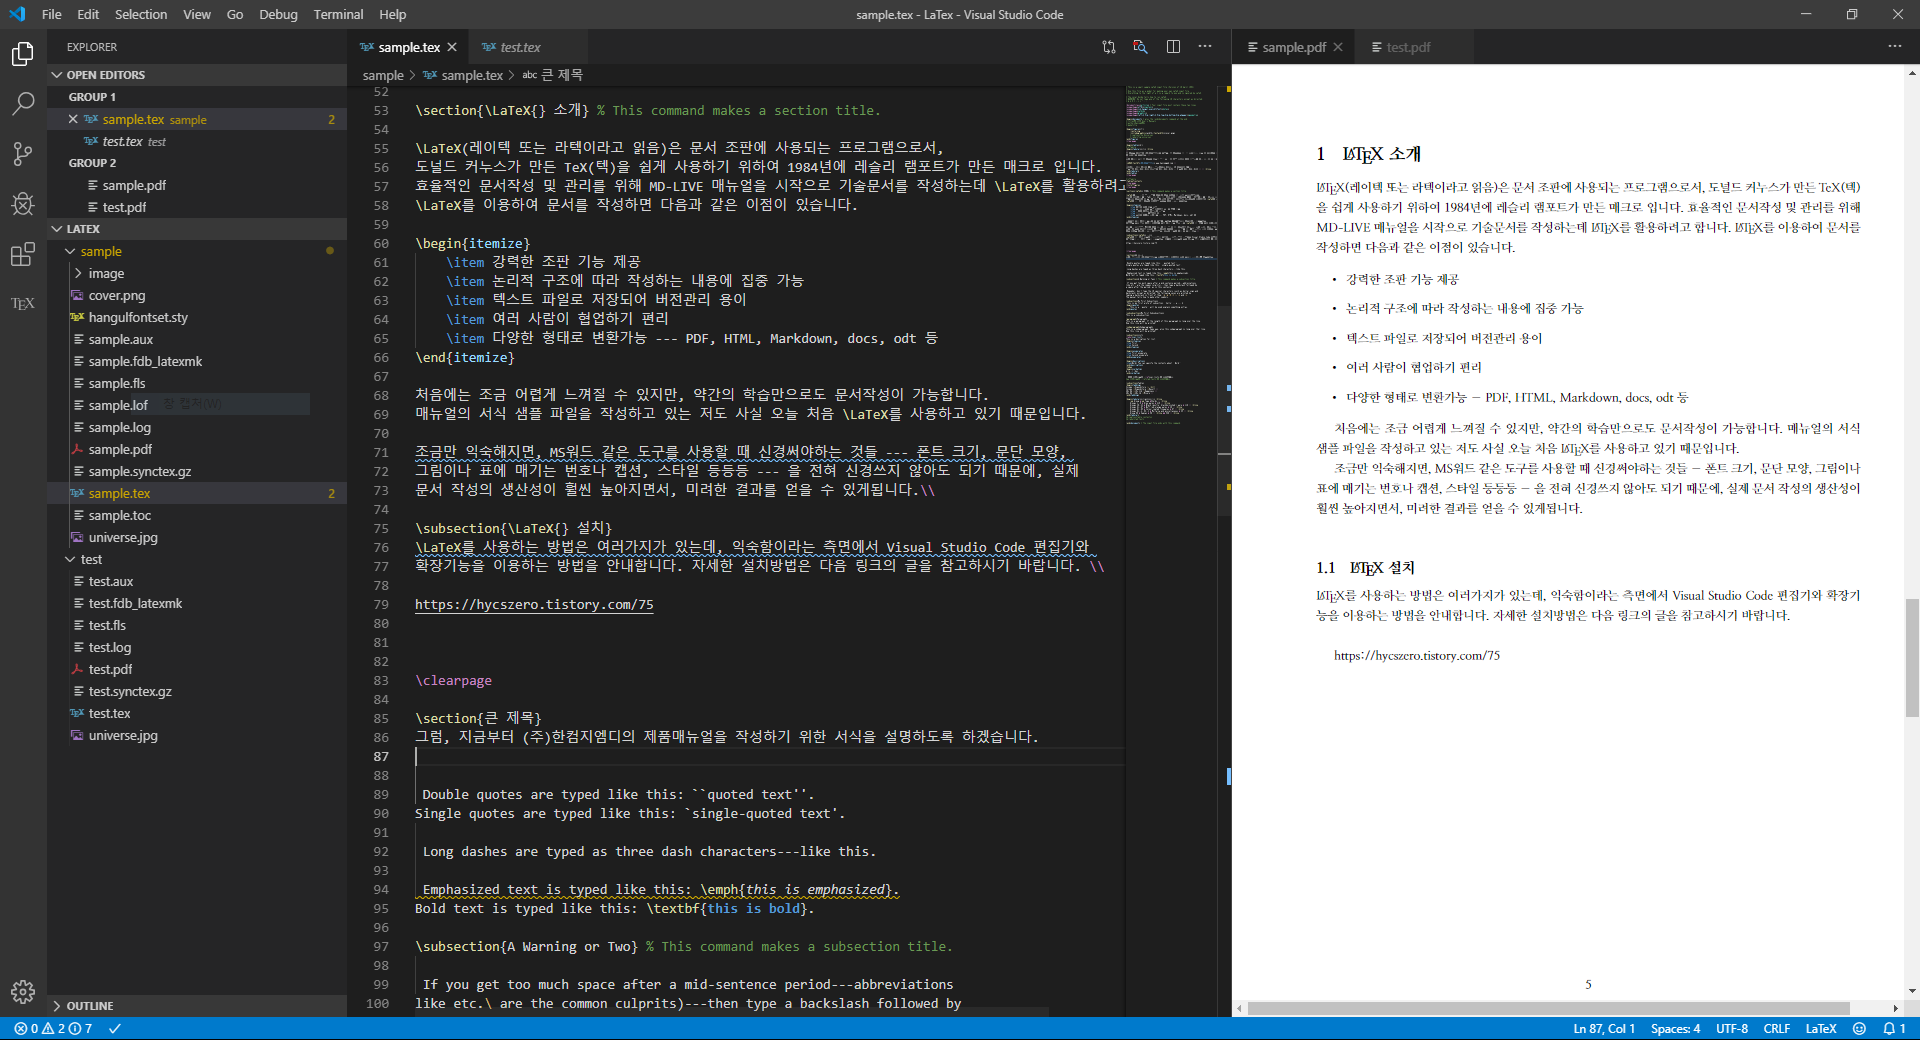
\includegraphics[scale=0.3]{images/chapter1/vscode.png}
    \caption{VS Code를 이용한 \LaTeX 편집}
    \label{fig:vscode}
\end{figure}

\section{\LaTeX{} 참고 자료}
\LaTeX의 기본적인 사용법은 다음 한국TEX사용자그룹(www.ktug.org)의 처음시작하기 문서를 참고하시기 바랍니다. \\

http://wiki.ktug.org/wiki/wiki.php/처음시작하기 \\
\clearpage

